\section{Graphentheorie}\label{kapitel:Graphentheorie}
Die Graphentheorie ist ein relativ junges Teilgebiet der Mathematik, aber dafür eines mit vielen praktischen Anwendungen. Auch in der Mathematik-Olympiade kommt Graphentheorie regelmäßig vor. In diesem Kapitel werden wir einige grundlegende Begriffe einführen. Die Beispielaufgaben sollen euch überdies dabei helfen, einige Beweistechniken aus der Kombinatorik zu wiederholen.

\subsection*{Grundlegende Begriffe}
Ein \emph{Graph} $G=(V,E)$ besteht aus einer Menge $V$ von Knoten und einer Menge~$E$ von Kanten, wobei jede Kante zwischen zwei Knoten verläuft. Dabei darf es zwischen zwei Knoten auch mehrere Kanten geben und es darf auch Kanten geben, die einen Knoten mit sich selbst verbinden. In diesem Fall sprechen wir von \emph{parallelen Kanten} und \emph{Schleifen}. Ein Graph ohne parallele Kanten und ohne Schleifen heißt \emph{schlicht} (der unten abgebildete Graph ist also nicht schlicht). Eine Kante $e$ zwischen zwei Knoten $u$ und $v$ notieren wir oft als $e=uv$. Wenn $G$ nicht schlicht ist, ist diese Notation etwas ungenau, denn $e$ wird dann nicht eindeutig durch $u$ und $v$ bestimmt. In der Praxis führt das aber so gut wie nie zu Verwirrung.

\begin{figure}[ht]
	\centering
	\begin{tabularx}{\textwidth}{X c X c X}
		& 
		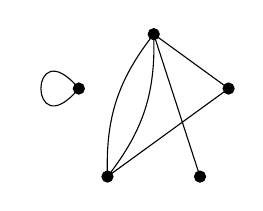
\begin{tikzpicture}
			\coordinate (a) at (18:1);
			\coordinate (b) at (90:1);
			\coordinate (c) at (162:1);
			\coordinate (d) at (234:1);
			\coordinate (e) at (306:1);
			\draw (c) to[in=130,out=230,loop,min distance=10mm,looseness=10] (c);
			\draw (a) to (b) to (e);
			\draw (a) to (d) to[bend left=20] (b) to[bend left=20] (d); 
			\draw[fill=black] (a) circle (2pt);
			\draw[fill=black] (b) circle (2pt);
			\draw[fill=black] (c) circle (2pt);
			\draw[fill=black] (d) circle (2pt);
			\draw[fill=black] (e) circle (2pt);
		\end{tikzpicture} & & \begin{tikzpicture}
		\coordinate (a) at (18:1);
		\coordinate (b) at (90:1);
		\coordinate (c) at (162:1);
		\coordinate (d) at (234:1);
		\coordinate (e) at (306:1);
		\path (a) edge[in=-50,out=50,loop,min distance=10mm,looseness=10,decoration={markings, mark=at position 0.55 with {\arrow{>}}},postaction={decorate}] (a);
		\path[decoration={markings, mark=at position 0.5 with {\arrow{>}}}] 
		(a) edge[postaction={decorate}] (b)
		(b) edge[postaction={decorate}] (c)
		(b) edge[postaction={decorate}] (d)
		(d) edge[postaction={decorate}] (a)
		(d) edge[postaction={decorate}] (c)
		(b) edge[postaction={decorate}] (e);
		\draw[fill=black] (a) circle (2pt);
		\draw[fill=black] (b) circle (2pt);
		\draw[fill=black] (c) circle (2pt);
		\draw[fill=black] (d) circle (2pt);
		\draw[fill=black] (e) circle (2pt);
		\end{tikzpicture} & \\\addlinespace
		& ein Graph $G_1$ & & ein gerichteter Graph $G_2$ & 
	\end{tabularx}
\end{figure}


In einem \emph{gerichteten Graphen} ist jede Kante außerdem mit einer Richtung ausgestattet. In einem gerichteten Graphen schreiben wir immer noch $e=uv$, um zu verdeutlichen, dass $e$ von $u$ nach $v$ verläuft. Im Gegensatz zu ungerichteten Graphen ist in dieser Schreibweise die Reihenfolge von $u$ und $v$ relevant. 

Wenn wir im Folgenden einfach nur \emph{Graph} schreiben, dann ist damit stets ein ungerichteter Graph gemeint. Außerdem beschränken wir uns auf \emph{endliche} Graphen, also solche bei denen die Mengen der Knoten $V$ und Kanten $E$ beide endlich sind.

Weiterhin gelten folgende Definitionen:

\textbf{Teilgraphen.} Ein \emph{Teilgraph} $G'=(V',E')$ eines Graphen $G=(V,E)$ ist ein Graph, dessen Knoten und Kanten in $G$ enthalten sind. Es muss also $V' \subseteq V$ und $E'\subseteq E$ gelten.

\textbf{Knotengrad.} In einem Graphen ist der \emph{Grad} $d(v)$ eines Knoten $v$  die Anzahl der angrenzenden Kanten. Dabei zählen Schleifen doppelt. In einem gerichteten Graphen ist der \emph{Ausgangsgrad} $d^+(v)$ die Anzahl der von $v$ ausgehenden Kanten und der \emph{Eingangsgrad} $d^-(v)$ die Anzahl der in $v$ eingehenden Kanten. Die Knoten, die mit $v$ durch eine Kante verbunden sind werden auch \emph{Nachbarn} von $v$ genannt.
	
\textbf{Wege, Pfade und Kreise.} Ein \emph{Weg} $W_n=v_1v_2\ldots v_n$ mit $n$ Knoten ist ein Graph mit den Knoten $v_1,v_2,\dotsc,v_n$ und den Kanten $v_iv_{i+1}$ für $i=1,2,\dotsc,n-1$. Ein \emph{Pfad} $P_n$ mit $n$ Knoten ist ein Weg, in dem kein Knoten doppelt vorkommt. Ein \emph{Kreis} $C_n$ der Länge $n$ ist ein Pfad $P_{n}$ zusammen mit der Kante $v_nv_1$. Ebenso lassen sich \emph{gerichtete Wege}, \emph{gerichtete Pfade} und \emph{gerichtete Kreise} definieren.
Wenn für einen Graphen $G=(V,E)$ von einem \emph{Weg/Pfad/Kreis in $G$} die Rede ist, so ist damit stets ein Teilgraph von~$G$ gemeint, der ein Weg/Pfad/Kreis ist.
	
\textbf{Zusammenhang.} Ein Graph heißt \emph{zusammenhängend}, wenn es zu je zwei Knoten immer einen Weg gibt, der diese beiden miteinander verbindet. Ein Graph heißt \emph{kreisfrei}, wenn er keinen Kreis als Teilgraph besitzt (der oben abgebildete ungerichtete Graph $G_1$ ist weder zusammenhängend noch kreisfrei).

Jeder Graph~$G$ lässt sich in zusammenhängende Teilgraphen zerlegen. Diese werden \emph{Zusammenhangskomponenten von~$G$} genannt. In vielen Aufgaben könnt ihr jede Zusammenhangskomponente einzeln behandeln und die Aufgabe so auf den Fall reduzieren, dass der betrachtete Graph zusammenhängend ist.
	
\textbf{Bäume.} Ein \emph{Baum} ist ein Graph, der zusammenhängend und kreisfrei ist. Ein Knoten $v$ in einem Baum ist ein \emph{Blatt} falls $d(v)=1$. Bei einem gerichteten Graphen reden wir von einem Baum, wenn der unterliegende ungerichtete Graph ein Baum ist und außerdem $d^-(v)\leqslant 1$ für alle Knoten $v\in V$ gilt. Ein Knoten mit $d^-(v)=0$ heißt \emph{Wurzel}.
\begin{figure}[ht]
	\centering
	\begin{tabularx}{\textwidth}{X c X c X}
		& 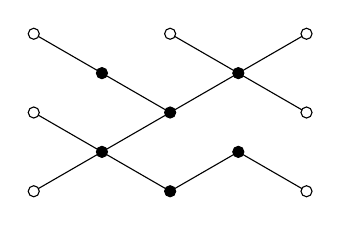
\begin{tikzpicture}
			\coordinate (a) at (-1.732,2);
			\coordinate (b) at (-1.732,1);
			\coordinate (c) at (-1.732,0);
			\coordinate (d) at (-0.866,1.5);
			\coordinate (e) at (-0.866,0.5);
			\coordinate (f) at (0,2);
			\coordinate (g) at (0,1);
			\coordinate (h) at (0,0);
			\coordinate (i) at (0.866,1.5);
			\coordinate (j) at (0.866,0.5);
			\coordinate (k) at (1.732,2);
			\coordinate (l) at (1.732,1);
			\coordinate (m) at (1.732,0);
			\draw (c) to (e) to (h) to (j) to (m);
			\draw (b) to (e) to (g) to (i) to (l);
			\draw (f) to (i) to (k);
			\draw (a) to (d) to (g); 
			\draw[fill=white] (a) circle (2pt);
			\draw[fill=white] (b) circle (2pt);
			\draw[fill=white] (c) circle (2pt);
			\draw[fill=black] (d) circle (2pt);
			\draw[fill=black] (e) circle (2pt);
			\draw[fill=white] (f) circle (2pt);
			\draw[fill=black] (g) circle (2pt);
			\draw[fill=black] (h) circle (2pt);
			\draw[fill=black] (i) circle (2pt);
			\draw[fill=black] (j) circle (2pt);
			\draw[fill=white] (k) circle (2pt);
			\draw[fill=white] (l) circle (2pt);
			\draw[fill=white] (m) circle (2pt);
		\end{tikzpicture} & & \begin{tikzpicture}
			\coordinate (a) at (-1.732,2);
			\coordinate (b) at (-1.732,1);
			\coordinate (c) at (-1.732,0);
			\coordinate (d) at (-0.866,1.5);
			\coordinate (e) at (-0.866,0.5);
			\coordinate (f) at (0,2);
			\coordinate (g) at (0,1);
			\coordinate (h) at (0,0);
			\coordinate (i) at (0.866,1.5);
			\coordinate (j) at (0.866,0.5);
			\coordinate (k) at (1.732,2);
			\coordinate (l) at (1.732,1);
			\coordinate (m) at (1.732,0);
			\path[decoration={markings, mark=at position 0.5 with {\arrow{>}}}] 
			(i) edge[postaction={decorate}] (g)
			(g) edge[postaction={decorate}] (d)
			(d) edge[postaction={decorate}] (a);
			\path[decoration={markings, mark=at position 0.5 with {\arrow{>}}}] 
			(i) edge[postaction={decorate}] (k);
			\path[decoration={markings, mark=at position 0.5 with {\arrow{>}}}]
			(i) edge[postaction={decorate}] (f);
			\path[decoration={markings, mark=at position 0.5 with {\arrow{>}}}]
			(i) edge[postaction={decorate}] (l);
			\path[decoration={markings, mark=at position 0.5 with {\arrow{>}}}] 
			(g) edge[postaction={decorate}] (e)
			(e) edge[postaction={decorate}] (h)
			(h) edge[postaction={decorate}] (j)
			(j) edge[postaction={decorate}] (m);
			\path[decoration={markings, mark=at position 0.5 with {\arrow{>}}}]
			(e) edge[postaction={decorate}] (b);
			\path[decoration={markings, mark=at position 0.5 with {\arrow{>}}}]
			(e) edge[postaction={decorate}] (c);
			\draw[fill=black] (a) circle (2pt);
			\draw[fill=black] (b) circle (2pt);
			\draw[fill=black] (c) circle (2pt);
			\draw[fill=black] (d) circle (2pt);
			\draw[fill=black] (e) circle (2pt);
			\draw[fill=black] (f) circle (2pt);
			\draw[fill=black] (g) circle (2pt);
			\draw[fill=black] (h) circle (2pt);
			\draw[fill=white] (i) circle (2pt);
			\draw[fill=black] (j) circle (2pt);
			\draw[fill=black] (k) circle (2pt);
			\draw[fill=black] (l) circle (2pt);
			\draw[fill=black] (m) circle (2pt);
		\end{tikzpicture} & \\
		& Ein Baum mit Blättern & & Ein gerichteter Baum mit Wurzel &
	\end{tabularx}
\end{figure}	
	
\textbf{Bipartite Graphen.} Ein Graph $G=(V,E)$ heißt \emph{bipartit}, wenn sich die Knotenmenge von $G$ so in zwei disjunkte Teilmengen $A$ und $B$ zerlegen lässt, dass nur Kanten zwischen $A$ und $B$ verlaufen, aber keine Kanten innerhalb von $A$ oder innerhalb von $B$. Die disjunkte Zerlegung $V=A\cup B$ wird auch \emph{Bipartition} genannt.
\begin{figure}[ht]
	\centering
	\begin{tabularx}{\textwidth}{X c X c X c X}
		& 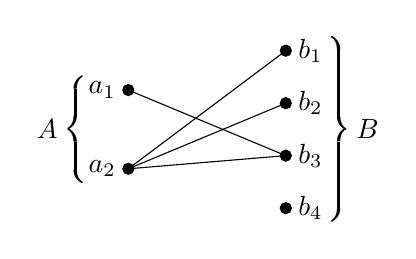
\begin{tikzpicture}
			\draw[fill=black] (0,0) circle (2pt) node[left=0.1em] {$a_1$};
			\draw[fill=black] (0,-1) circle (2pt) node[left=0.1em] {$a_2$};
			\draw[fill=black] (2,0.5) circle (2pt) node[right=0.1em] {$b_1$};
			\draw[fill=black] (2,-0.167) circle (2pt) node[right=0.1em] {$b_2$};
			\draw[fill=black] (2,-0.833) circle (2pt) node[right=0.1em] {$b_3$};
			\draw[fill=black] (2,-1.5) circle (2pt) node[right=0.1em] {$b_4$};
			\draw (0,0) -- (2,-0.833);
			\draw (0,-1) -- (2,-0.167);
			\draw (0,-1) -- (2,0.5);
			\draw (0,-1) -- (2,-0.833);
			\path (0,0) -- (0,-1) node[pos=0.5, left=2.2em] {$A$} node[pos=0.5, below=1.2em, sloped] {$\underbrace{\hspace{1.35cm}}$};
			\path (2,-1.5) -- (2,0.5) node[pos=0.5,right=2.2em] {$B$} node[pos=0.5, below=1.2em, sloped] {$\underbrace{\hspace{2.35cm}}$};
		\end{tikzpicture} & & 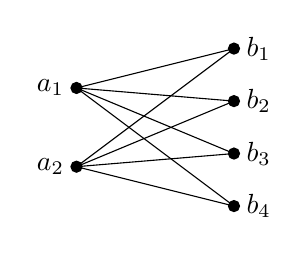
\begin{tikzpicture}
			\draw[fill=black] (0,0) circle (2pt) node[left=0.1em] {$a_1$};
			\draw[fill=black] (0,-1) circle (2pt) node[left=0.1em] {$a_2$};
			\draw[fill=black] (2,0.5) circle (2pt) node[right=0.1em] {$b_1$};
			\draw[fill=black] (2,-0.167) circle (2pt) node[right=0.1em] {$b_2$};
			\draw[fill=black] (2,-0.833) circle (2pt) node[right=0.1em] {$b_3$};
			\draw[fill=black] (2,-1.5) circle (2pt) node[right=0.1em] {$b_4$};
			\draw (0,0) -- (2,-0.833);
			\draw (0,0) -- (2,0.5);
			\draw (0,0) -- (2,-0.167);
			\draw (0,0) -- (2,-1.5);
			\draw (0,-1) -- (2,-0.833);
			\draw (0,-1) -- (2,0.5);
			\draw (0,-1) -- (2,-0.167);
			\draw (0,-1) -- (2,-1.5);
		\end{tikzpicture} & & 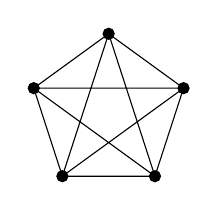
\begin{tikzpicture}
		\coordinate (a) at (18:1);
		\coordinate (b) at (90:1);
		\coordinate (c) at (162:1);
		\coordinate (d) at (234:1);
		\coordinate (e) at (306:1);
		\draw (a) to (b) to (c) to (d) to (e) to (a);
		\draw (a) to (c) to (e) to (b) to (d) to (a);
		\draw[fill=black] (a) circle (2pt);
		\draw[fill=black] (b) circle (2pt);
		\draw[fill=black] (c) circle (2pt);
		\draw[fill=black] (d) circle (2pt);
		\draw[fill=black] (e) circle (2pt);
		\end{tikzpicture} &\\
		& bipartiter Graph & & vollständiger bipatiter & & vollständiger Graph $K_5$ & \\
		& & &  Graph $K_{2,4}$ & & &
		\end{tabularx} 
	\end{figure}	
	
\textbf{Vollständige Graphen.} Der \emph{vollständige Graph $K_n$} ist ein Graph mit $n$ Knoten, in dem jeder Knoten mit jedem anderen verbunden ist. Der \emph{vollständige bipartite Graph $K_{m,n}$} ist ein bipartiter Graph mit $\abs{A}=m$, $\abs{B}=n$, in dem jeder Knoten aus $A$ mit jedem Knoten aus $B$ verbunden ist.
	
\textbf{Planare Graphen.} Ein \emph{planarer Graph} ist ein Graph, der so auf ein Blatt Papier gezeichnet kann, dass sich keine zwei Kanten schneiden. Jede Kante darf dabei beliebig krumm sein, aber sie darf keine Lücken enthalten. Zum Beispiel sind alle Bäume planare Graphen. 
\begin{figure}[ht]
	\centering
	\begin{tabularx}{\textwidth}{X c X c X}
		& 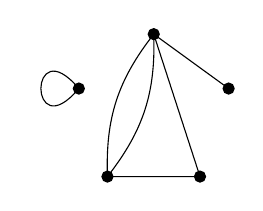
\begin{tikzpicture}
			\coordinate (a) at (18:1);
			\coordinate (b) at (90:1);
			\coordinate (c) at (162:1);
			\coordinate (d) at (234:1);
			\coordinate (e) at (306:1);
			\draw (c) to[in=130,out=230,loop,min distance=10mm,looseness=10] (c);
			\draw (a) to (b) to (e);
			\draw (e) to (d) to[bend left=20] (b) to[bend left=20] (d); 
			\draw[fill=black] (a) circle (2pt);
			\draw[fill=black] (b) circle (2pt);
			\draw[fill=black] (c) circle (2pt);
			\draw[fill=black] (d) circle (2pt);
			\draw[fill=black] (e) circle (2pt);
		\end{tikzpicture} & & 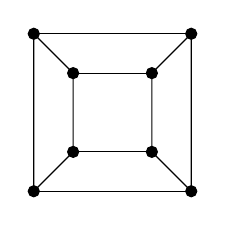
\begin{tikzpicture}
			\coordinate (a) at (0,0);
			\coordinate (b) at (0,2);
			\coordinate (c) at (2,2);
			\coordinate (d) at (2,0);
			\coordinate (e) at (0.5,0.5);
			\coordinate (f) at (0.5,1.5);
			\coordinate (g) at (1.5,1.5);
			\coordinate (h) at (1.5,0.5);
			\draw (a) to (e) to (f) to (b) to (a);
			\draw (c) to (d) to (h) to (g) to (c);
			\draw (a) to (d);
			\draw (b) to (c);
			\draw (f) to (g);
			\draw (e) to (h);
			\draw[fill=black] (a) circle (2pt);
			\draw[fill=black] (b) circle (2pt);
			\draw[fill=black] (c) circle (2pt);
			\draw[fill=black] (d) circle (2pt);
			\draw[fill=black] (e) circle (2pt);
			\draw[fill=black] (f) circle (2pt);
			\draw[fill=black] (g) circle (2pt);
			\draw[fill=black] (h) circle (2pt);
		\end{tikzpicture} &  \\
		& $G_1$ als planarer Graph & & Ein Würfel als planarer Graph &
	\end{tabularx} 
\end{figure}	
	
Wie man in diesem Beispielbild seht, ist der Graph $G_1$ planar, obwohl er oben mit einer Überschneidung gezeichnet wurde.

\subsection*{Beispielaufgaben zur Graphentheorie}
Hier sind einige sehr interessante Resultate aus der Graphentheorie, die auch in Olympiade-Aufgaben weiterhelfen können. In Graphentheorie-Aufgaben kommt es sehr häufig vor, dass mit Induktion über die Menge der Knoten oder Kanten argumentiert wird. Auch Algorithmen kommen sehr prominent zum Einsatz; in Kapitel~\ref{kapitel:Algorithmen}: \emph{Algorithmen in der Kombinatorik} wird auf dieses Thema für allgemeine Aufgaben im Detail eingegangen. Ansonsten braucht ihr natürlich auch die Standardmethoden\footnote{Wenn ihr eine schnelle Wiederholung zu diesen Themen wollt, dann sei euch das Buch \emph{Geometria -- Scientiae Atlantis~1} von Eckard Specht und Robert Strich ans Herz gelegt. Dieses Buch enthält nicht nur, wie der Name nahelegt, jede Menge interessante Geometrie, sondern auch sehr praktische Zusammenfassungen zu anderen olympiaderelevanten Themen. Ihr könnt es relativ kostengünstig hier bestellen: \url{http://hydra.nat.uni-magdeburg.de/math4u/fix/bestellung.html}.} in der Kombinatorik, wie das Schubfachprinzip, das Extremalprinzip und das Invarianzprinzip.
\begin{aufgabe*}\label{aufgabe:Handschlagslemma}
	Beweise das Handschlagslemma. Folgere, dass in jedem Graphen die Anzahl der Knoten von ungeradem Grad gerade sein muss.
	\begin{satzmitnamen}[Handschlagslemma]
		In jedem Graphen $G=(V,E)$ gilt
		\begin{equation*}
			\sum_{v\in V} d(v) = 2\abs{E}\,.
		\end{equation*}
		In jedem gerichteten Graphen $G=(V,E)$ gilt
		\begin{equation*}
			\sum_{v\in V}d^+(v)=\sum_{v\in V}d^-(v)=\abs{E}\,
		\end{equation*}
	\end{satzmitnamen}
\end{aufgabe*}
\begin{aufgabe*}\label{aufgabe:Blatt}
	\begin{enumerate}
		\item \label{teilaufgabe:BaumHatBlaetter}Zeige, dass jeder Baum mit mindestens zwei Knoten mindestens ein Blatt hat.
		\item \label{teilaufgabe:BaumKnotenKanten}Beweise: Für jeden Baum $G=(V,E)$ gilt $\abs{E} = \abs{V} -1$. Folgere, dass jeder Baum mit $\abs*{V}\geqslant 2$ sogar mindestens zwei Blätter hat.
	\end{enumerate}
\end{aufgabe*}
\begin{aufgabe*}\label{aufgabe:Bipartit}
	Beweise, dass ein Graph $G=(V,E)$ genau dann bipartit ist, wenn es in $G$ keine Kreise von ungerader Länge gibt.
\end{aufgabe*}
\begin{aufgabe*}\label{aufgabe:Schlicht}
	Beweise, dass in jedem schlichten Graphen (mit mindestens zwei Knoten) zwei Knoten existieren, die den gleichen Grad haben.
\end{aufgabe*}
\begin{aufgabe*}[*]\label{aufgabe:Euler-Hierholzer}
	Beweise den Satz von Euler-Hierholzer.
	\begin{satzmitnamen}[Satz von Euler-Hierholzer]
		In einem zusammenhängenden Graphen $G=(V,E)$ existiert genau dann ein Weg, der jede Kante genau einmal durchläuft, wenn $G$ höchstens zwei Knoten mit ungeradem Grad besitzt. Ferner existiert genau dann ein geschlossener Weg \embrace{also ein Weg, dessen Anfangs- und Endknoten übereinstimmen}, der alle Kanten durchläuft, wenn alle Knoten in $G$ geraden Grad haben.
	\end{satzmitnamen}
\end{aufgabe*}

Ein solcher Weg wird auch als \emph{Eulerweg} bezeichnet. Die Frage, ob für einen gegebenen Graphen ein Eulerweg existiert, ist auch als \enquote{Königsberger Brückenproblem} bekannt. 

\begin{aufgabe*}[*]\label{aufgabe:Polyeder}
	Beweise den Eulerschen Polyedersatz:
	\begin{satzmitnamen}[Eulerscher Polyedersatz]
		Sei $G$ ein planarer Graph. Sei $Z$ die Menge der Zusammenhangskomponenten von~$G$ und sei $F$ die Menge der Flächen in einer überschneidungsfreien Zeichnung von~$G$ \embrace{die \enquote{unendlich große Fläche außenrum} wird mitgezählt}. Dann gilt stets:
		\begin{equation*}
			\abs{V}-\abs{E}+\abs*{F} = \abs*{Z}+1\,.
		\end{equation*}
	\end{satzmitnamen}
\end{aufgabe*}
\begin{aufgabe*}[*]\label{aufgabe:Unplanar}
	Zeige, dass die vollständigen Graphen $K_5$ und $K_{3,3}$ nicht planar sind.
\end{aufgabe*}
\begin{aufgabe*}[**]\label{aufgabe:Dirac}
	Beweise den Satz von Dirac:
	\begin{satzmitnamen}[Satz von Dirac]
		Sei $G=(V,E)$ ein schlichter Graph mit $n=\abs*{V}$ Knoten. Wenn jeder Knoten $v\in V$ einen Grad $d(v)\geqslant n/2$ hat, dann gibt es in $G$ einen Kreis, der durch jeden Knoten genau einmal geht.
	\end{satzmitnamen}
\end{aufgabe*}
Ein solcher Kreis wird auch~\emph{Hamiltonkreis genannt}. Im Gegensatz zu Eulerwegen, für deren Existenz es ein sehr einfaches hinreichendes und notwendiges Kriterium gibt (wie wir in Aufgabe~\ref{aufgabe:Euler-Hierholzer} gesehen haben), ist es im Allgemeinen sehr kompliziert zu entscheiden, ob ein gegebener Graph~$G$ einen Hamiltonkreis enthält.

\vfill\hrule\vspace{-1em}

\subsection*{Tipps zu den Beispielaufgaben}
\textbf{Tipp zu Aufgabe~\ref{aufgabe:Handschlagslemma}.} Der Grund für den Namen \enquote{Handschlagslemma} ist folgender: Stell dir vor, eine Menge $V$ von sehr wichtigen Leuten trifft sich zu einer sehr wichtigen Konferenz. Einige davon begrüßen einander mit Händeschütteln. Aus Infektionsschutzgründen soll jeder Teilnehmende~$v$ am Ende angeben, wie viele Hände er geschüttelt hat. Außerdem gibt es eine Infektionsschutzbeauftragte, die sehr aufmerksam zählt, wie viele Handschläge stattfinden.

\textbf{Tipps zu Aufgabe~\ref{aufgabe:Blatt}.} Beweise~\ref{teilaufgabe:BaumHatBlaetter} durch Widerspruch.

Für~\ref{teilaufgabe:BaumKnotenKanten} benutze~\ref{teilaufgabe:BaumHatBlaetter} und schneide sukzessive Blätter ab.
	
\textbf{Tipp zu Aufgabe~\ref{aufgabe:Bipartit}.} Überlegen dir zuerst, warum ein Graph mit einem ungeraden Kreis nicht bipartit sein kann. Kannst du dein Argument umdrehen und ein Verfahren angeben, mit dem zu jedem Graphen ohne ungeraden Kreis eine Bipartition konstruiert werden kann?

\textbf{Tipp zu Aufgabe~\ref{aufgabe:Schlicht}.}
Wie groß kann $d(v)$ maximal sein, sodass der Graph schlicht bleibt? Angenommen, es gäbe einen Graphen der schlicht ist und bei dem jeder Knoten einen unterschiedlichen Grad hat. Was kannst du in diesem Fall über die $d(v)$ aussagen?

\textbf{Tipp zu Aufgabe~\ref{aufgabe:Euler-Hierholzer}.}
Der schwierige Teil der Aufgabe besteht darin, zu zeigen, dass in einem Graphen mit lauter geraden Knotengraden auch tatsächlich ein geschlossener Eulerweg existiert.  Benutze dafür Induktion über die Anzahl der Kanten.

\textbf{Tipp zu Aufgabe~\ref{aufgabe:Polyeder}.} Diese Aufgabe lässt sich auf verschiedene Art und Weise mit Induktion lösen. Pass dabei auf, dass dein Argument keine Fälle übersieht.

\textbf{Tipp zu Aufgabe~\ref{aufgabe:Unplanar}.} Benutze den Eulerschen Polyedersatz. Wie viele Kanten haben die Flächen in $K_5$ mindestens? Wie viele in $K_{3,3}$?

\textbf{Tipps zu Aufgabe~\ref{aufgabe:Dirac}.} Wenn es ein Gegenbeispiel gäbe es auch auch ein Gegenbeispiel~$G$ mit maximal vielen Kanten.

Verbinde zwei Knoten in~$G$, die noch nicht verbunden waren. Danach gibt es einen Hamiltonkreis (überlege dir, warum). Benutze das Schubfachprinzip, um diesen Hamiltonkreis zu einem Hamiltonkreis in~$G$ umzubauen.


